% METODOLOGIA------------------------------------------------------------------

\chapter{Metodologia}
\label{chap:metodologia}

A metodologia foi dividia nos passos mostrados na Figura \ref{dia:metodologia}. O primeiro passo realizado no trabalho foi a criação da base de vídeos, usando a base UCF50 - Action Recognition Data Set \cite{reddy2013recognizing}. Sobre os vídeos foram aplicadas 14 distorções descritas na Seção~\ref{sec:ataques}, em seguida, foram geradas as assinaturas utilizando os algoritmos de diferença de quadro, gradientes, medida ordinal, quadros de cena, padrão binário por região e wavelets, descritos no Capítulo~\ref{chap:revisao}. Foram então realizados procedimentos para definição de parâmetros para os métodos usando um subconjunto dos vídeos. Por fim, foi elaborada a análise comparativa dos resultados obtidos em um segundo subconjunto. Estes resultados serão discutidos em detalhes no Capítulo \ref{chap:resultados}. As seções a seguir detalham cada um dos passos.

% \begin{description}
% \item[Etapa 1] Aquisição da base de vídeos UCF50 - Action Recognition Data Set \citeauthor{reddy2013recognizing}.
% \item[Etapa 2] Aplicação das 14 distorções descritas na Seção~\ref{sec:ataques} sobre a base.
% \item[Etapa 3] Geração das assinaturas utilizando os algoritmos baseados em diferença de quadro, gradientes, medida ordinal, quadros de cena, padrão binário por região e wavelets, descritos no Capítulo~\ref{chap:revisao}.
% \item[Etapa 4] Realização do procedimento de comparação de um conjunto de treinamento das assinaturas, a fim de definir um limiar para classificação.
% \item[Etapa 5] Realização do procedimento de comparação de um conjunto de testes das assinaturas, a partir dos limiares obtidos na Etapa 4.
% \item[Etapa 5] Análise comparativa dos resultados obtidos a partir da Etapa 4. Os resultados desta etapa serão discutidos em detalhes no próximo capítulo.
% \end{description}

\begin{figure}[h]
    \centering
    \caption{Diagrama das Etapas de Desenvolvimento.}
    \label{dia:metodologia}
    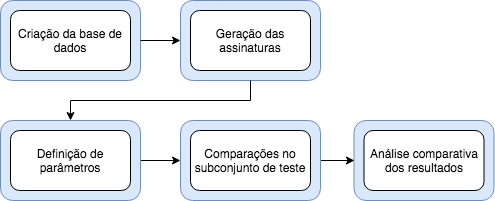
\includegraphics[width=0.8\textwidth]{dados/figuras/diagramas/Diag-Metodologia}
    \fonte{Autoria própria.}
\end{figure}

\section{Criação da Base de Vídeos}
\label{sec:database}

Para a realização dos experimentos desta monografia, foi escolhida a base de vídeos UCF50 - Action Recognition Data Set \cite{reddy2013recognizing}, que é comumente utilizada em projetos de reconhecimento de movimento humano. Ela foi escolhida pela quantidade de vídeos que contém, sua licença de livre utilização e a possibilidade de cortar um única cena, que permite uma comparação fácil, já que não é preciso procurar uma cena em um vídeo longo.

A base contém 50 categorias diferentes que representam ações do quotidiano, como por exemplo ciclismo, natação, caminhada com o cachorro, TaiChi, etc. Dentro de cada categoria, há pelo menos 4 vídeos pertencentes a uma mesma gravação, apresentando assim os mesmos personagens, fundo e ponto de vista. A fim de reduzir o número de vídeos que apresentam o mesmo conteúdo, foram selecionados apenas o primeiro vídeo de cada grupo.

A base original é composta de 6.681 vídeos com duração média entre 3 a 9 segundos. Após a seleção descrita no parágrafo anterior restaram 1.264 vídeos. Para cada vídeo selecionado foram aplicadas as distorções descritas na Seção~\ref{sec:ataques}, totalizando 18.960 vídeos, sendo destes, 17.696 vídeos resultantes das distorções. A Figura~\ref{fig:exemplos} apresenta alguns exemplos de vídeos da base.

\begin{figure}
    \centering
    \caption{Exemplos de vídeos retirados da base. O primeiro mostra um jogo de beisebol, o segundo mostra uma criança fazendo malabarismo, o terceiro mostra uma competição de levantamento de pesos.}
    \label{fig:exemplos}
    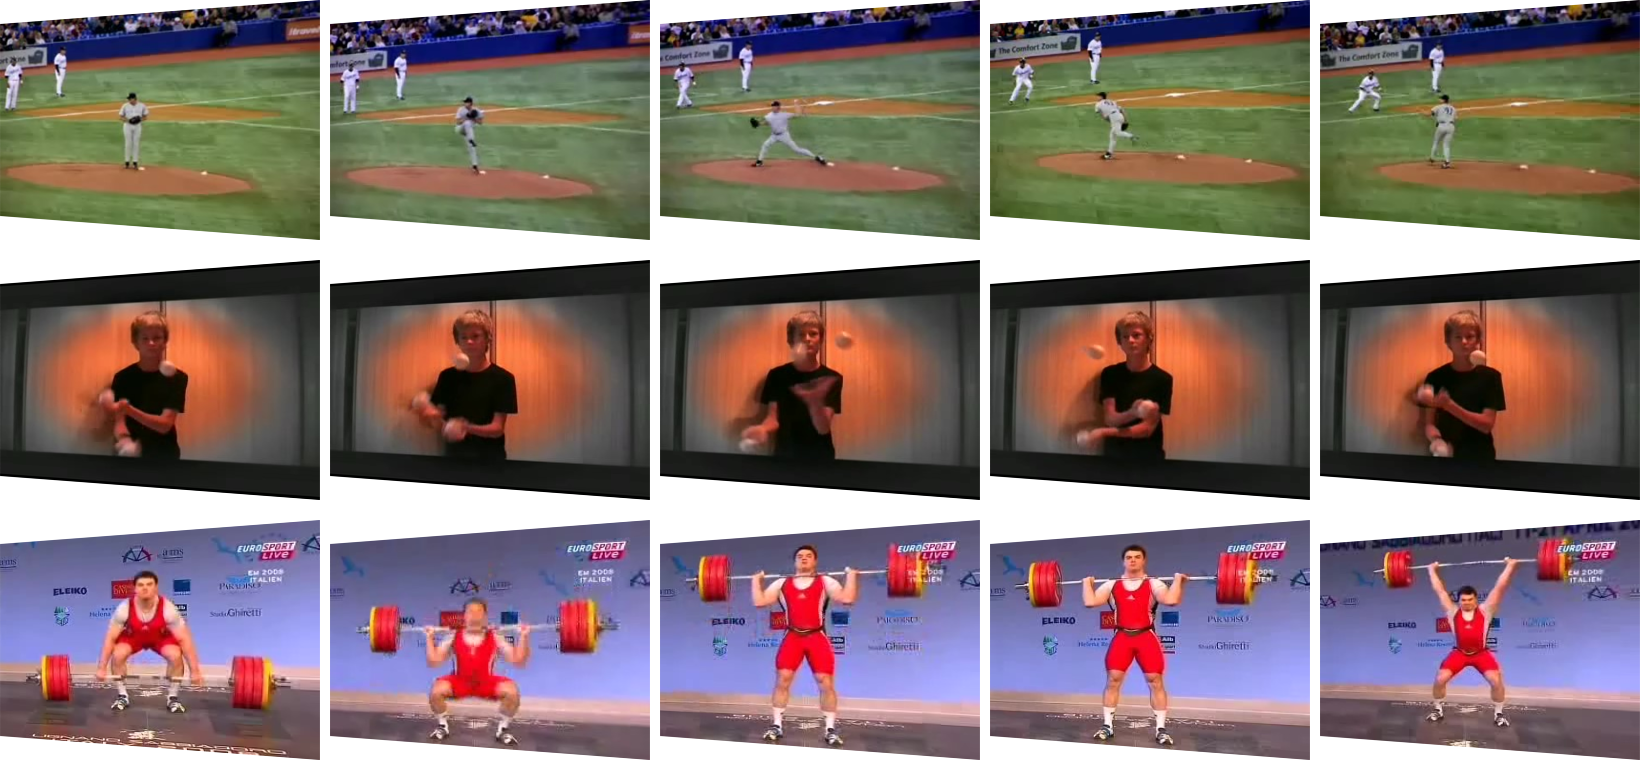
\includegraphics[width=0.8\textwidth]{dados/figuras/exemplos}
    \fonte{Autoria própria.}
\end{figure}

Estes cenários propiciam a avaliação do desempenho das diferentes assinaturas revisadas neste trabalho quanto à robustez e a unicidade, e para garantir a reprodutibilidade do experimento, os parâmetros utilizados para a aplicação de cada uma das distorções são explicitados na Tabela~\ref{tab:params}. Para facilitar a discussão dos resultados, serão utilizadas as siglas definidas na primeira coluna da tabela quando houver referência às distorções.

\begin{table}[!ht]
\centering
\caption{Parâmetros usados na aplicação das distorções.}
\label{tab:params}
\begin{tabular}{|p{0.2\textwidth}|p{0.4\textwidth}|p{0.4\textwidth}|} \hline
    \textbf{Sigla} & \textbf{Distorção} & \textbf{Parâmetros} \\ \hline
    TEXT & Adição de texto e legendas &  Texto: "Testing descriptor for scene" \\ \hline
    WATERMARK & Adição de marca d'água & \begin{tabular}{@{}l@{}}Texto: "Copyright"\\ Tamanho da fonte: 20\\ Opacidade: 65\% \end{tabular}\\ \hline
    BORDER & Adição de bordas & Tamanho da borda: 25 pixels \\ \hline
    BIG & Redimensionamento da altura e largura dos vídeos & \begin{tabular}{@{}l@{}} Fator de redimensionamento: 2\\ Mantém aspect ratio: sim \end{tabular} \\ \hline
    SMALL & Redimensionamento da altura e largura dos vídeos& \begin{tabular}{@{}l@{}} Fator de redimensionamento: 2\\ Mantém aspect ratio: sim \end{tabular} \\ \hline
    CROP & Recorte de uma faixa ou região dos quadros & Largura máxima: 620 Altura Máxima: 338 Ponto de recorte X: 107 Ponto de recorte Y: 107 \\ \hline
    FLOP & Inversão/espelhamento & Sentido: horizontal \\ \hline
    ROTATE & Rotação & 10 graus \\ \hline
    BLUR & Desfoque & \begin{tabular}{@{}l@{}}Tipo: gaussiano\\ Sigma: 3\end{tabular} \\ \hline
    COLOR & Inversão das cores &  \\ \hline
    JPEG & Alteração das compressão dos quadros do vídeo & Apenas 20\% da qualidade \\ \hline
    FAST1 & Aceleração do vídeo 1 & Aumento da velocidade em 50\% \\ \hline
    FAST2 & Aceleração do vídeo 2 & Aumento da velocidade em 25\% \\ \hline
    FRAME & Remoção de Frames & Remoção de 20\% \\ \hline
\end{tabular}
\end{table}

\section{Geração das Assinaturas}
\label{sec:met-assinaturas}

O passo final de preparação para os experimentos deste trabalho foi a criação das assinaturas utilizando os 6 algoritmos descritos no Capítulo~\ref{chap:revisao}. As assinaturas foram geradas para todos os 17.696 vídeos originais e distorcidos, totalizando 106.176 assinaturas. Para facilitar a realização dos experimentos, todas as assinaturas foram armazenadas em um banco de dados juntamente com: os dados do vídeo usados para computar a assinatura, se o vídeo é um vídeo original ou um distorcido, o tipo da distorção e uma referência ao vídeo original, além do tipo de assinatura utilizado. A Tabela~\ref{tab:assinaturas} apresenta todas as assinaturas sendo utilizadas, além dos tipos de características de um vídeo utilizados para obtê-las. A primeira coluna da tabela apresenta a sigla de cada assinatura que será utilizada no Capítulo \ref{chap:resultados}. Todas as assinaturas foram normalizadas para o intervalod $[0 - 1]$.

% junto do intervalo numérico em que as assinaturas se encontram,

\begin{table}[h]
    \centering
    \caption{Assinaturas utilizadas para comparação.}
    \label{tab:assinaturas}
    \begin{tabular}{|p{0.2\textwidth}|p{0.259\textwidth}|p{0.259\textwidth}|} \hline
        \textbf{Sigla} & \textbf{Assinatura} & \textbf{Características} \\ \hline
        gradient & Gradiente & - \\ \hline
        framedif & FrameDiff & - \\ \hline
        medidaordina & Medida Ordinal & - \\ \hline
        wavelet & Wavelets & - \\ \hline
        rb & RBP & - \\ \hline
        sceneframe & Scene Frame & - \\ \hline
    \end{tabular}
\end{table}

As assinaturas geradas nesta etapa foram arranjadas em grupos de parametrização e testes para a realização do experimento. 

Para a criação de um caso de teste, é escolhida uma assinatura do grupo de assinaturas originais e uma assinatura do grupo de teste, sempre geradas pelo mesmo algoritmo como pode ser visto da Figura \ref{fig:comparacao}, e estas são comparadas segundo o método descrito na Seção~\ref{sec:met-comparacao}. Caso o resultado da comparação fique abaixo de um limiar empiricamente definido, o vídeo que gerou a assinatura de teste é considerado como uma cópia do vídeo que gerou a assinatura original.

\begin{figure}
    \centering
    \caption{Diagrama das comparações dos casos de teste}
    \label{fig:comparacao}
    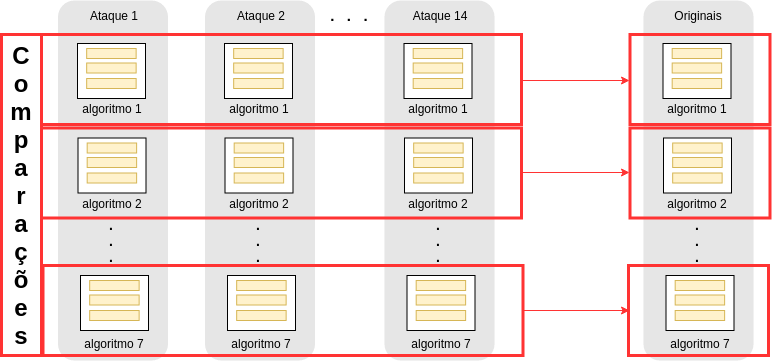
\includegraphics[width=0.8\textwidth]{dados/figuras/Comparador-1}
    \fonte{Autoria própria}
\end{figure}

Para classificar se uma assinatura do grupo de teste é uma cópia de uma assinatura do grupo de originais, é preciso definir um parâmetro de corte para cada algoritmo. Para isso, foi definido um cenário de treinamento de 8.848 vídeos por algoritmo, ou seja, metade do total de assinaturas respectivas a cada algoritmo. Isso representa um total de 53.088 vídeos que são realmente cópias, enquanto 


em que 50\% das combinações de assinatura que são cópias foram escolhidos aleatoriamente, ou seja, 8.848 por algoritmo, totalizando 53.088 casos de treinamento de cópias. O mesmo número de casos de treinamento de não-cópias foi escolhido aleatoriamente.

\section{Comparação de Assinaturas}
\label{sec:met-comparacao}

As assinaturas geradas na etapa anterior são compostas de vetores de características e cada um dos trabalhos descreve uma forma de compará-los, geralmente utilizando a distância Euclidiana ou a distância de Manhattan. Para simplificar a implementação e análise dos resultados, foi necessária a escolha de uma medida única capaz de lidar com as características de cada assinatura. Um dos fatores a ser considerado é que o tamanho das assinaturas é proporcional ao tamanho dos vídeos dos quais elas provém, além disso, este trabalho usa algumas distorções do tipo temporal que alteram a velocidade e o \textit{framerate} de vídeos, alterando seu tamanho. Sendo assim, a medida utilizada precisa lidar com assinaturas de tamanhos e frequências diferentes.

Enquanto a distância Euclidiana pode ser útil para comparar as assinaturas de um único quadro de cada vídeo, o fato dela comparar cada valor de duas assinaturas de um em um a torna suscetível a distorções temporais. Para resolver os problemas mencionados, foi escolhido o DTW (\textit{Dynamic Time Warping}) como forma de comparação, uma técnica conhecida para alinhamento entre duas sequências temporais \cite{muller2007dynamic}. Originalmente, esta técnica foi utilizada para a comparação de diferentes padrões vocais em aplicações de reconhecimento de voz, mas o DTW já foi utilizado com sucesso para lidar com deformações temporais e velocidades diferentes em dados dependentes de tempo, explica \citeonline{muller2007dynamic}. A Figura \ref{fig:dist-comparacao} mostra um comparativo entre o funcionamento da distância Euclidiana e do DTW, nota-se o pareamento um para um da distância Euclidiana (imagem de cima), e o pareamento $n$ para um do DTW.

\begin{figure}[h]
    \centering
    \caption{Distância entre duas sequências temporais medida usando distância Euclidiana (na imagem de cima) e o DTW (na imagem de baixo).}
    \fonte{\cite{muller2007dynamic}.}
    \label{fig:dist-comparacao}
    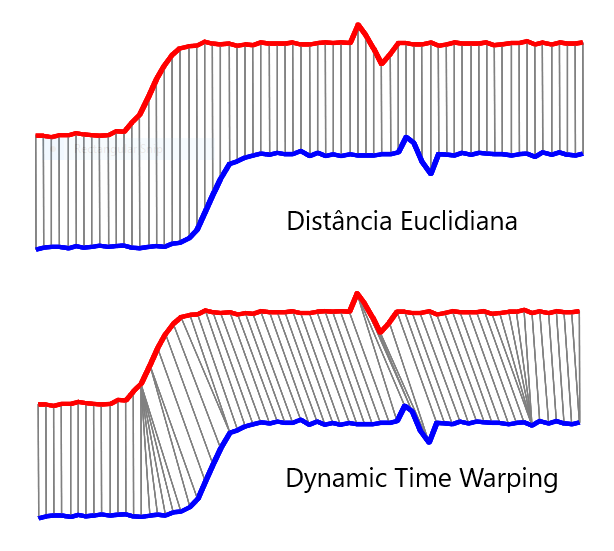
\includegraphics[width=0.6\textwidth]{dados/figuras/dtw-euclidiana}
\end{figure}

Para achar esse pareamento, o DTW compara todos os valores das duas sequências temporais utilizando uma medida de distância (normalmente a distância Manhattan ou Euclidiana) como parâmetro, como mostra a Figura \ref{fig:dtw-caminho}. Em seguida, percorre-se a matriz da última célula até a primeira, sempre escolhendo a célula com o menor custo como próximo passo. O caminho formado é o pareamento entre valores das duas sequências temporais. Sua saída é um valor numérico que é relativo à medida de distância escolhida como parâmetro. É necessário calcular um limiar para utilizar o resultado da comparação do algoritmo, sendo que os valores menores que o limiar representam que há similaridade entre as duas sequências comparadas \cite{muller2007dynamic}.


\begin{figure}[h]
    \centering
    \caption{a) Matriz de custo formada comparando duas sequências temporais. b) Caminho com menor custo.}
    \label{fig:dtw-caminho}
    \begin{tabular}{ll}
    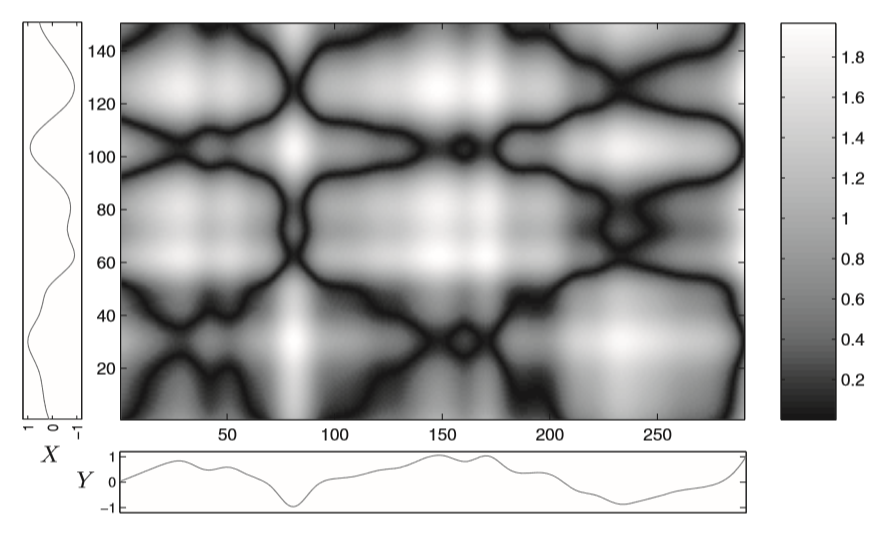
\includegraphics[width=0.4\textwidth]{dados/figuras/dtw-comparacao} &
    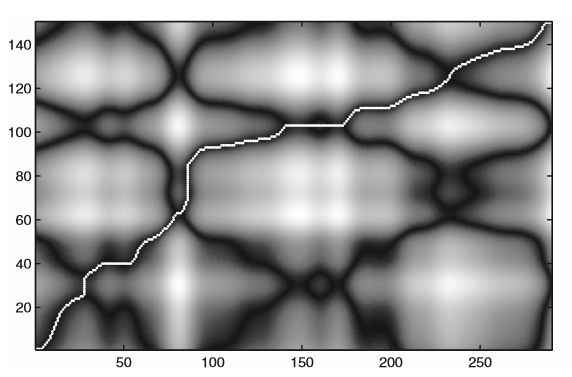
\includegraphics[width=0.4\textwidth]{dados/figuras/dtw-comparacao-caminho} \\
    a) Matriz de custo & b) Caminho mais barato
    \end{tabular}
    \fonte{\cite{muller2007dynamic}.}
\end{figure}

% Fórmula do DTW

Em sua forma original, o DTW tem uma complexidade de $ O(N^{2}) $, por esse motivo, foi utilizada uma variante do algoritmo chamada FastDTW, que provem alinhamentos ótimos ou quase ótimos com complexidade de $O(N)$.

% falar que precisa normalizar

\section{Experimentos}
\label{sec:met-Experimentos}

Os experimentos realizados neste trabalho são dividos em duas etapas: a obtenção dos parâmetros de cada assinatura para a classificação de cópias (treinamento), e testes das assinaturas. Para a criação dos casos de treinamento/teste, são necessárias algumas definições. O conjunto $A_o = \{a_1, a_2, a_3, ..., a_n\}$ contém todas as $n$ assinaturas dos vídeos originais, o conjunto $A_d = \{a_1, a_2, a_3, ..., a_m\}$ contém as $m$ assinaturas dos vídeos distorcidos. Como há 1.264 vídeos originais na base de vídeos e 7 tipos de assinaturas sendo examinadas neste trabalho, o conjunto $A_o$ tem tamanho $n=8.848$. Como há 14 distorções sendo utilizadas neste trabalho, o conjunto $A_d$ tem tamanho $m=123.872$.

Para cada assinatura distorcida $a \in A_d$, existe uma assinatura correspondente $b \in A_o$ tal que $a$ seja uma cópia distorcida de $b$. Um caso de treinamento/teste $c$ é composto de uma tupla $(a, b)$ tal que $a \in A_o$ e $b \in A_d$. Um caso de treinamento $c$ é marcado como "cópia" se $b$ for uma cópia distorcida de $a$, senão é marcado como "não cópia". Sendo assim, há um total de 22.367.744 de possíveis casos de treinamento/teste para cada tipo de assinatura, sendo apenas 17.584 marcados como "cópia". Visando a criação de um conjunto de casos de treinamento balanceado, foram escolhidos aleatoriamente 50\% dos 17.584 casos de "cópia" (8.792), e o mesmo número de casos "não cópia" para cada algoritmo. O mesmo critério foi utilizado para a criação dos conjuntos de teste: o resto dos 50\% dos casos "cópia" foi selecionado, além de 8.792 casos "não cópia".

\begin{figure}[h]
    \centering
    \caption{Diagrama da divisão dos casos de teste para parametrização e testes.}
    \label{fig:casosteste}
  
    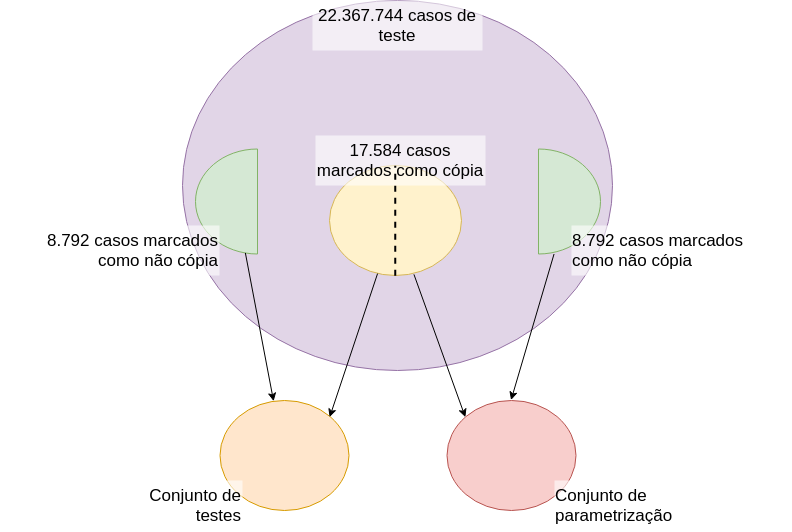
\includegraphics[width=0.8\textwidth]{dados/figuras/Casos}
    
      \fonte{Autoria própria.}
    
\end{figure}

% \begin{table}[h]
%     \centering
%     \begin{tabular}{|l|l|l|l|l|}
%         \hline
%         Casos Total & Casos "cópia" & Casos "não cópia" & Casos "cópia" para treinamento & Casos "não cópia" para treinamento \\ \hline
%         22.367.744 & 17.584 & 22.350.160 & 8.792 & 8.792 \\ \hline
%     \end{tabular}
% \end{table}



Para realizar uma classificação de um vídeo de teste como sendo cópia de um dos vídeos originais, as assinaturas dos dois são comparadas utilizando o DTW (definido da Seção~\ref{sec:met-comparacao}), que retorna como resultado uma medida de distância. Essa classificação utilizando o valor de distância só é possível após definido um limiar de corte para cada algoritmo, sendo que um vídeo de teste é considerado cópia de um vídeo original se a distância entre os dois obtida através do DTW esteja abaixo deste limiar. Logo, a primeira etapa dos experimentos é a definição destes limiares de forma empírica.

O conjunto de parametrização definido anteriormente é divido em 5 subconjuntos organizados de forma aleatória. Para cada subconjunto, é simulada a classificação de "cópia" e "não-cópia" com um intervalo de valores, a fim de encontrar um limiar ideal. Com o intuito de maximizar o número de verdadeiros-positivos e diminuir o número de falsos-negativos, é utilizada a medida \textit{FMeasure} como parâmetro, escolhendo o limiar que maximiza este valor. Ao final da simulação para os 5 subconjuntos, o limiar final de cada assinatura é definido como a média dos limiares obtidos com a simulação para cada subconjunto.

Na fase de testes, são utilizados os limiares encontrados na fase de parametrização para classificar os conjuntos de teste e avaliar cada tipo de assinatura quanto à sua robustez e unicidade quando usadas individualmente. Por fim, é realizada a combinação das assinaturas "gradiente", "wavelets", "medida ordinal", "scene frame" e "rbp", com a assinatura "camera motion" para avaliar se a combinação de assinaturas temporais e espaciais é mais eficaz na detecção de cópias.
